\documentclass{exam}
\usepackage{tasks}

\usepackage{amsmath,amssymb,amsfonts}
\usepackage{graphicx}
\usepackage{amsthm}
\usepackage[french]{babel}
\usepackage{enumitem}
\usepackage{currfile}
\usepackage{tikz}
\usetikzlibrary{babel,arrows, arrows.meta,calc,fit,patterns,plotmarks,shapes.geometric,shapes.misc,shapes.symbols,shapes.arrows,shapes.callouts, shapes.multipart, shapes.gates.logic.US,shapes.gates.logic.IEC, er, automata,backgrounds,chains,topaths,trees,petri,mindmap,matrix, calendar, folding,fadings,through,positioning,scopes,decorations.fractals,decorations.shapes,decorations.text,decorations.pathmorphing,decorations.pathreplacing,decorations.footprints,decorations.markings,shadows}
\usepackage{tkz-base}
\usepackage{tkz-euclide}
\usepackage{qrcode}
\usepackage{mathrsfs}
\usepackage{enumitem}
\usepackage[french]{babel}
\setlength{\parindent}{0cm}

\usepackage{multicol}
\newenvironment{clist}{\begin{center}\begin{inparaenum}}{\end{inparaenum}\end{center}}

\pagestyle{empty}
\graphicspath{ {../../Images/} }
\input{\currfiledir ../def.tex}
\def \Document {Contrôle 2}

\usepackage{geometry}
\geometry{left=1.5cm, right=1.5cm, top=1.5cm, bottom=1.5cm}

\makeatletter
\def\gap#1{%
  \setbox\@tempboxa\hbox{{\color{white}#1}}%
  \@tempdima\wd\@tempboxa
  \rlap{\unhbox\@tempboxa}%
  \hb@xt@\@tempdima{\dotfill}%
}
\makeatother   

\theoremstyle{definition}
\newtheorem{exercice}{Exercice}

\begin{document}
\large

\noindent{
\makebox[0pt][l]{\textbf{\Niveau}}%
\makebox[\textwidth][c]{\textbf{\Chapitre}}%
\makebox[0pt][r]{\textbf{\Document\ (A) -- 30min}}
}

\vspace{2mm}

\noindent{\makebox[\textwidth]{Nom et prénom:\enspace\hrulefill}}

\vspace{2mm}

% Exercice 1
\begin{exercice}~\\
	\begin{minipage}[t]{0.5\textwidth}%
        \vspace{-\topskip}	
        À l'aide de la figure ci-contre, donner un vecteur égal aux sommes de vecteurs suivantes :
        \begin{enumerate}
            \item \makebox[3.5cm]{$\overrightarrow{OC} + \overrightarrow{BA}$} $= {\makebox[5em]{\enspace\hrulefill}}$
            %\item \makebox[3.5cm]{$\overrightarrow{DF} + \overrightarrow{OE}$} $= {\makebox[5em]{\enspace\hrulefill}}$
            %\item \makebox[3.5cm]{$\overrightarrow{AO} + 2 \overrightarrow{BO} + \overrightarrow{EB}$} $= {\makebox[5em]{\enspace\hrulefill}}$
            \item \makebox[3.5cm]{$\overrightarrow{ED} - \overrightarrow{FD} + \overrightarrow{AE}$} $= {\makebox[5em]{\enspace\hrulefill}}$
            %\item \makebox[3.5cm]{$-\overrightarrow{BD} + \overrightarrow{OD} + \overrightarrow{OC}$} $= {\makebox[5em]{\enspace\hrulefill}}$
        \end{enumerate}
	\end{minipage}
	\begin{minipage}[t]{0.5\textwidth}%	
        \vspace{-\topskip}
        \begin{center}
            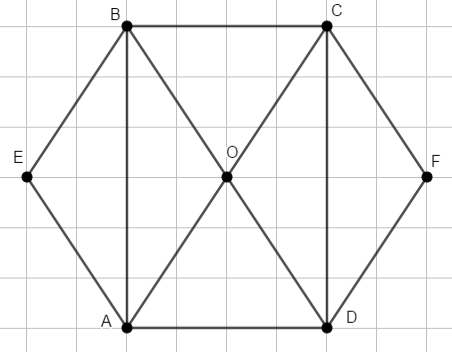
\includegraphics[width=0.7\linewidth]{cflash_7.png}
        \end{center}
	\end{minipage}
\end{exercice}

\vfill

% Exercice 2
\begin{exercice}
    Simplifier, à l'aide de la relation de Chasles, les expressions suivantes :
    \begin{tasks}[style=enumerate](2)
        \task $\overrightarrow{IP} + \overrightarrow{MI}$
        \task $\overrightarrow{JI} - \overrightarrow{JK} + \overrightarrow{IK}$
        %\task $-\overrightarrow{MN} + \overrightarrow{NP} + \overrightarrow{MP}$
    \end{tasks}
    \framebox[1\textwidth]{\parbox{1\textwidth}{
        \begin{tasks}[style=enumerate](2)
            \task
            \task
            %\task
        \end{tasks}
    \vspace{6em}}}
\end{exercice}


% % Exercice 3
% \begin{exercice}~\\
% 	\begin{minipage}[t]{0.65\textwidth}%
%         \vspace{-\topskip}	
%         Soient $ABCD$ et $ABEF$ deux parallélogrammes comme représentés sur la figure ci-contre.
%         \begin{enumerate}
%             \item Donner deux vecteurs égaux à $\overrightarrow{AB}$.
%             \item Quelle est la nature de $CDFE$ ? Justifier.
%         \end{enumerate}
% 	\end{minipage}
% 	\begin{minipage}[t]{0.35\textwidth}%	
%         \vspace{-\topskip}
%         \begin{center}
%             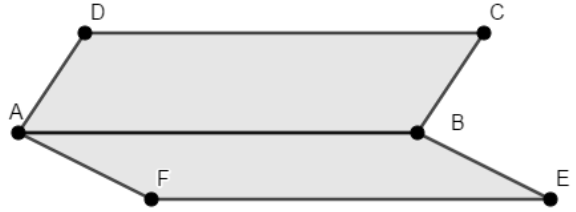
\includegraphics[width=0.9\linewidth]{swappy-20250103_142842.png}
%         \end{center}
% 	\end{minipage}
%     \vspace{1em}
% 
%     \framebox[1\textwidth]{\parbox{1\textwidth}{
%         \begin{enumerate}
%             \item 
%             \item 
%         \end{enumerate}
%     \vspace{4em}}}
% \end{exercice}

\vfill

\begin{exercice}{}{}


~\\
 \begin{minipage}[t]{0.5\linewidth} Construire le point $R$ tel que $\overrightarrow{TR} = \vec{u} + \vec{v}$.

\begin{tikzpicture}[baseline={(current bounding box.north)}, scale=0.35]
%
\tkzInit[xmin=-9.9, xmax=9.9, ymin=-9.9, ymax=9.9]
\tkzGrid[thin,color=lightgray]
%\tkzAxeXY
% Vecteur 1
% %Segment 1
% \draw[color={rgb,255:red,241; green,89; blue,41},line width=3, ->, >=stealth] (0, 0) -- (1, 0);
% % Vecteur 2
% %Segment 2
% \draw[color={rgb,255:red,241; green,89; blue,41},line width=3, ->, >=stealth] (0, 0) -- (0, 1);
% Point T
\draw[line width=1] plot[mark=x, mark size=0.230769cm] coordinates{(-5,5)};
\node[color=black,line width=1,above right] at (-5,5) {$T$};
% Vecteur $\vec{\vec{u}}$
\node[color=black,line width=1] at (-1.209381,2.906867) {$\vec{u}$};
%Segment 3
\draw[color=black,line width=1, ->, >=stealth] (-5, 5) -- (2, 0);
% Vecteur $\vec{\vec{v}}$
\node[color=black,line width=1] at (-2.543094,0.703069) {$\vec{v}$};
%Segment 4
\draw[color=black,line width=1, ->, >=stealth] (-5, 5) -- (-1, -4);
% Point T
\draw[line width=1] plot[mark=x, mark size=0.230769cm] coordinates{(-5,5)};
\node[color=black,line width=1,above right] at (-5,5) {$T$};
\end{tikzpicture} \end{minipage}
% @see : https://coopmaths.fr/alea?uuid=6cf42&id=2G23-2&n=1&d=10&s=3&alea=Scml&cd=1&cols=2
\begin{minipage}[t]{0.5\linewidth} Construire le point $D$ tel que $\overrightarrow{TD} = \vec{u} + \vec{v}$.

\begin{tikzpicture}[baseline={(current bounding box.north)}, scale=0.35]
%
\tkzInit[xmin=-9.9, xmax=9.9, ymin=-9.9, ymax=9.9]
\tkzGrid[thin,color=lightgray]
% Vecteur 1
% Point T
\draw[line width=1] plot[mark=x, mark size=0.230769cm] coordinates{(-2,0)};
\node[color=black,line width=1,above right] at (-2,0) {$T$};
% Vecteur $\black
\node[color=black,line width=1] at (2.456906,-1.296931) {$\vec{u}$};
%Segment 3
\draw[color=black,line width=1, ->, >=stealth] (0, 3) -- (4, -6);
% Vecteur $\black
\node[color=black,line width=1] at (2.5,3.5) {$\vec{v}$};
%Segment 4
\draw[color=black,line width=1, ->, >=stealth] (3, 1) -- (3, 6);
% Point T
\draw[line width=1] plot[mark=x, mark size=0.230769cm] coordinates{(-2,0)};
\node[color=black,line width=1,above right] at (-2,0) {$T$};
\end{tikzpicture}
\end{minipage}
\end{exercice}

\newpage

\begin{center}
\begin{tikzpicture}[scale=0.8]
  \draw[gray!30,very thin,step=0.5] (0,0) grid (14,9);
\draw[-{Latex[length=2.5mm]},thick] (4,7) -- (1,4) node[above left] {$\vec u$};
  \draw[-{Latex[length=2.5mm]},thick] (1,8) -- (3.5,8) node[above,midway] {$\vec v$};
  \node at (8,8) {$\times$};
  \node[right] at (8.15,8) {$A$};
\end{tikzpicture}
\end{center}

\begin{exercice}{}{}
On considère deux vecteurs $\vec u$ et $\vec v$. $A$ est un point donné.
\begin{enumerate}[label=\arabic*.]
\item Construire les points $B$ et $C$ tels que :
  \begin{tasks}[label=\textbullet](2)
  \task $\overrightarrow{AB}=\vec u+\vec v$
  \task $\overrightarrow{AC}=\vec u-\vec v$.
  \end{tasks}
\item Construire les points $P$, $Q$ et $R$ tels que :
  \begin{tasks}[label=\textbullet](3)
  \task $\overrightarrow{BP}=\dfrac13\vec u$
  \task $\overrightarrow{PQ}=-2\vec v$
  \task $\overrightarrow{QR}=\dfrac{-1}{3}\vec u$.
  \end{tasks}
\item Que constate-t-on à propos des points $C$ et $R$ ? Le justifier par un calcul vectoriel.
\end{enumerate}
    \framebox[1\textwidth]{\parbox{1\textwidth}{
    \vspace{28em}}}
\end{exercice}

% Exercice 4
% \begin{exercice}
%     On a placé trois points $A$, $B$ et $C$ dans le graphique ci-dessous.
%     \begin{center}
%         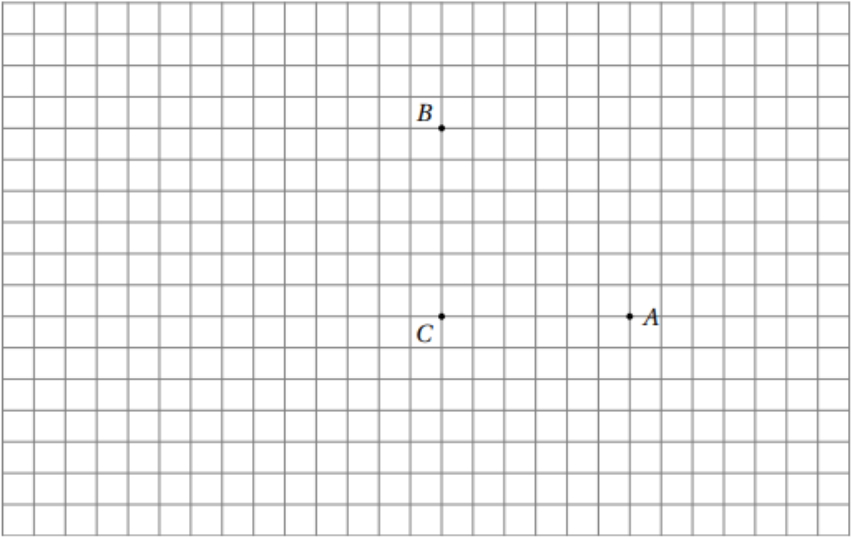
\includegraphics[width=0.6\textwidth]{swappy-20250103_143242.png}
%     \end{center}
%     \begin{enumerate}
%         \item Placer les points $I$, $J$, $K$ et $L$ définis par les égalités suivantes :
%         \[
%         \overrightarrow{AI} = \frac{1}{2} \overrightarrow{AB}, \quad 
%         \overrightarrow{BJ} = 2 \overrightarrow{BA}, \quad
%         \overrightarrow{CK} = -\frac{2}{3} \overrightarrow{CA}, \quad
%         \overrightarrow{CL} = \frac{2}{3} \overrightarrow{BC} - \frac{13}{6} \overrightarrow{BA}
%         \]
%         \item Tracer le quadrilatère $IJKL$. Que peut-on conjecturer sur sa nature ?
%             
%             \vspace{0.3em}
% 
%             \framebox[1\linewidth]{\parbox{1\linewidth}{
%                 % reponse
%             \vspace{1em}}}
%             
%         \item Nous allons démontrer la conjecture faite au point précédent.
%         \begin{enumerate}
%             \item À l'aide de la relation de Chasles, exprimer $\overrightarrow{IJ}$ en fonction de $\overrightarrow{AI}$, $\overrightarrow{AB}$ et $\overrightarrow{BJ}$. En déduire $\overrightarrow{IJ}$ en fonction de $\overrightarrow{AB}$.
%             
%             \vspace{0.3em}
% 
%             \framebox[1\linewidth]{\parbox{1\linewidth}{
%                 % reponse
%             \vspace{9em}}}
%             \item À l'aide de la relation de Chasles, exprimer $\overrightarrow{LK}$ en fonction de $\overrightarrow{CK}$ et $\overrightarrow{CL}$. Toujours à l'aide de la relation de Chasles, travailler l'expression précédente jusqu'à obtenir $\overrightarrow{LK}$ en fonction de $\overrightarrow{AB}$.
%             
%             \vspace{0.3em}
% 
%             \framebox[1\linewidth]{\parbox{1\linewidth}{
%                 % reponse
%             \vspace{9em}}}
%         \end{enumerate}
%         \item Conclure sur la nature de $IJKL$.
%             
%             \vspace{0.3em}
% 
%             \framebox[1\linewidth]{\parbox{1\linewidth}{
%                 % reponse
%             \vspace{3em}}}
%     \end{enumerate}
% \end{exercice}
% 
% \end{document}
% 
% % \begin{exercice}
% % 
% % Développer et réduire l'expression suivante.
% %  $A = (5c-9)(5c+9)$
% %     \begin{center}
% %         \framebox[1\textwidth]{\parbox{5.5in}{
% %             %\centering \underline{Réponse:}
% %         \vspace{6em}}}
% %     \end{center}
% % \end{exercice}
% % 
% % \begin{exercice}
% % 
% % Factoriser l'expression suivante.\begin{multicols}{2}
% %  \begin{minipage}[t]{\linewidth} $A = 3(x+1)+x(x+1)$ \end{minipage}
% % \end{multicols}
% %     \begin{center}
% %         \framebox[1\textwidth]{\parbox{4.5in}{
% %             %\centering \underline{Réponse:}
% %         \vspace{6em}}}
% %     \end{center}
% % \end{exercice}
% % 
% % \begin{exercice}
% % 
% %  Le nombre proposé existe-t-il ? Justifier.\begin{multicols}{2}
% %  \begin{minipage}[t]{\linewidth} $\sqrt{2-\pi}$ \end{minipage}
% % \end{multicols}
% % 	\framebox[1\textwidth]{\parbox{4.5in}{
% % 		%\centering \underline{Réponse:}
% % 	\vspace{6em}}}
% % \end{exercice}
% % 
% % \begin{exercice}
% % 
% % 
% %  Écrire à l'aide d'un seul vecteur :
% %         $\overrightarrow{EF}+\overrightarrow{FE}=${\makebox[5em]{\enspace\hrulefill}}
% % \end{exercice}
% % 
% % \begin{exercice}
% % 
% % 
% %  Sans justifier, donner l'image du point $O$ par la translation de vecteur $\overrightarrow{HB}$.
% %  
% %  \begin{minipage}[t]{0.5\linewidth}
% % 	\vspace{-\topskip}
% %  \begin{tikzpicture}[baseline,scale = 0.7]
% % 
% %     \tikzset{
% %       point/.style={
% %         thick,
% %         draw,
% %         cross out,
% %         inner sep=0pt,
% %         minimum width=5pt,
% %         minimum height=5pt,
% %       },
% %     }
% %     \clip (-1,-1) rectangle (12,5);
% %     	\draw[color ={{black}},line width = 0.625,opacity = 0.8] (-0.1875,4.1875)--(0.1875,3.8125);\draw[color ={{black}},line width = 0.625,opacity = 0.8] (-0.1875,3.8125)--(0.1875,4.1875);\draw[color ={{black}},line width = 0.625,opacity = 0.8] (1.8125,4.1875)--(2.1875,3.8125);\draw[color ={{black}},line width = 0.625,opacity = 0.8] (1.8125,3.8125)--(2.1875,4.1875);\draw[color ={{black}},line width = 0.625,opacity = 0.8] (3.8125,4.1875)--(4.1875,3.8125);\draw[color ={{black}},line width = 0.625,opacity = 0.8] (3.8125,3.8125)--(4.1875,4.1875);\draw[color ={{black}},line width = 0.625,opacity = 0.8] (5.8125,4.1875)--(6.1875,3.8125);\draw[color ={{black}},line width = 0.625,opacity = 0.8] (5.8125,3.8125)--(6.1875,4.1875);\draw[color ={{black}},line width = 0.625,opacity = 0.8] (7.8125,4.1875)--(8.1875,3.8125);\draw[color ={{black}},line width = 0.625,opacity = 0.8] (7.8125,3.8125)--(8.1875,4.1875);\draw[color ={{black}},line width = 0.625,opacity = 0.8] (9.8125,4.1875)--(10.1875,3.8125);\draw[color ={{black}},line width = 0.625,opacity = 0.8] (9.8125,3.8125)--(10.1875,4.1875);\draw[color ={{black}},line width = 0.625,opacity = 0.8] (-0.1875,2.1875)--(0.1875,1.8125);\draw[color ={{black}},line width = 0.625,opacity = 0.8] (-0.1875,1.8125)--(0.1875,2.1875);\draw[color ={{black}},line width = 0.625,opacity = 0.8] (1.8125,2.1875)--(2.1875,1.8125);\draw[color ={{black}},line width = 0.625,opacity = 0.8] (1.8125,1.8125)--(2.1875,2.1875);\draw[color ={{black}},line width = 0.625,opacity = 0.8] (3.8125,2.1875)--(4.1875,1.8125);\draw[color ={{black}},line width = 0.625,opacity = 0.8] (3.8125,1.8125)--(4.1875,2.1875);\draw[color ={{black}},line width = 0.625,opacity = 0.8] (5.8125,2.1875)--(6.1875,1.8125);\draw[color ={{black}},line width = 0.625,opacity = 0.8] (5.8125,1.8125)--(6.1875,2.1875);\draw[color ={{black}},line width = 0.625,opacity = 0.8] (7.8125,2.1875)--(8.1875,1.8125);\draw[color ={{black}},line width = 0.625,opacity = 0.8] (7.8125,1.8125)--(8.1875,2.1875);\draw[color ={{black}},line width = 0.625,opacity = 0.8] (9.8125,2.1875)--(10.1875,1.8125);\draw[color ={{black}},line width = 0.625,opacity = 0.8] (9.8125,1.8125)--(10.1875,2.1875);\draw[color ={{black}},line width = 0.625,opacity = 0.8] (-0.1875,0.1875)--(0.1875,-0.1875);\draw[color ={{black}},line width = 0.625,opacity = 0.8] (-0.1875,-0.1875)--(0.1875,0.1875);\draw[color ={{black}},line width = 0.625,opacity = 0.8] (1.8125,0.1875)--(2.1875,-0.1875);\draw[color ={{black}},line width = 0.625,opacity = 0.8] (1.8125,-0.1875)--(2.1875,0.1875);\draw[color ={{black}},line width = 0.625,opacity = 0.8] (3.8125,0.1875)--(4.1875,-0.1875);\draw[color ={{black}},line width = 0.625,opacity = 0.8] (3.8125,-0.1875)--(4.1875,0.1875);\draw[color ={{black}},line width = 0.625,opacity = 0.8] (5.8125,0.1875)--(6.1875,-0.1875);\draw[color ={{black}},line width = 0.625,opacity = 0.8] (5.8125,-0.1875)--(6.1875,0.1875);\draw[color ={{black}},line width = 0.625,opacity = 0.8] (7.8125,0.1875)--(8.1875,-0.1875);\draw[color ={{black}},line width = 0.625,opacity = 0.8] (7.8125,-0.1875)--(8.1875,0.1875);\draw[color ={{black}},line width = 0.625,opacity = 0.8] (9.8125,0.1875)--(10.1875,-0.1875);\draw[color ={{black}},line width = 0.625,opacity = 0.8] (9.8125,-0.1875)--(10.1875,0.1875);
% % 	\draw [color={black}] (0,4.5) node[anchor = center,scale=1, rotate = 0] {A};
% % 	\draw [color={black}] (2,4.5) node[anchor = center,scale=1, rotate = 0] {B};
% % 	\draw [color={black}] (4,4.5) node[anchor = center,scale=1, rotate = 0] {C};
% % 	\draw [color={black}] (6,4.5) node[anchor = center,scale=1, rotate = 0] {D};
% % 	\draw [color={black}] (8,4.5) node[anchor = center,scale=1, rotate = 0] {E};
% % 	\draw [color={black}] (10,4.5) node[anchor = center,scale=1, rotate = 0] {F};
% % 	\draw [color={black}] (-0.5,2) node[anchor = center,scale=1, rotate = 0] {G};
% % 	\draw [color={black}] (1.5,1.5) node[anchor = center,scale=1, rotate = 0] {H};
% % 	\draw [color={black}] (3.5,1.5) node[anchor = center,scale=1, rotate = 0] {I};
% % 	\draw [color={black}] (5.5,1.5) node[anchor = center,scale=1, rotate = 0] {J};
% % 	\draw [color={black}] (7.5,1.5) node[anchor = center,scale=1, rotate = 0] {K};
% % 	\draw [color={black}] (10.5,2) node[anchor = center,scale=1, rotate = 0] {L};
% % 	\draw [color={black}] (0,-0.5) node[anchor = center,scale=1, rotate = 0] {M};
% % 	\draw [color={black}] (2,-0.5) node[anchor = center,scale=1, rotate = 0] {N};
% % 	\draw [color={black}] (4,-0.5) node[anchor = center,scale=1, rotate = 0] {O};
% % 	\draw [color={black}] (6,-0.5) node[anchor = center,scale=1, rotate = 0] {P};
% % 	\draw [color={black}] (8,-0.5) node[anchor = center,scale=1, rotate = 0] {Q};
% % 	\draw [color={black}] (10,-0.5) node[anchor = center,scale=1, rotate = 0] {R};
% % 	
% % 	\draw[color ={gray},opacity = 0.4] (0,0)--(0,4);
% % 	\draw[color ={gray},opacity = 0.4] (1,0)--(1,4);
% % 	\draw[color ={gray},opacity = 0.4] (2,0)--(2,4);
% % 	\draw[color ={gray},opacity = 0.4] (3,0)--(3,4);
% % 	\draw[color ={gray},opacity = 0.4] (4,0)--(4,4);
% % 	\draw[color ={gray},opacity = 0.4] (5,0)--(5,4);
% % 	\draw[color ={gray},opacity = 0.4] (6,0)--(6,4);
% % 	\draw[color ={gray},opacity = 0.4] (7,0)--(7,4);
% % 	\draw[color ={gray},opacity = 0.4] (8,0)--(8,4);
% % 	\draw[color ={gray},opacity = 0.4] (9,0)--(9,4);
% % 	\draw[color ={gray},opacity = 0.4] (10,0)--(10,4);
% % 	\draw[color ={gray},opacity = 0.4] (0,0)--(10,0);
% % 	\draw[color ={gray},opacity = 0.4] (0,1)--(10,1);
% % 	\draw[color ={gray},opacity = 0.4] (0,2)--(10,2);
% % 	\draw[color ={gray},opacity = 0.4] (0,3)--(10,3);
% % 	\draw[color ={gray},opacity = 0.4] (0,4)--(10,4);
% % 	\draw[color ={{blue}},line width = 1.25,opacity = 0.8] (3.8125,0.1875)--(4.1875,-0.1875);\draw[color ={{blue}},line width = 1.25,opacity = 0.8] (3.8125,-0.1875)--(4.1875,0.1875);
% % \end{tikzpicture}
% % \end{minipage}
% % \begin{minipage}[t]{0.5\linewidth}
% % 	\vspace{-\topskip}
% % 	\vspace{4.7em}
% % 	Réponse : {\makebox[5em]{\enspace\hrulefill}}
% % \end{minipage}
% % \end{exercice}
% % 
% % \newpage
% % 
% % \begin{exercice}~\\
% % 	\begin{minipage}[t]{0.4\textwidth}%
% % 	\vspace{-\topskip}	
% % 	Construire le point $H$ tel que $\overrightarrow{EH} = \vec{u} + \vec{v}$.
% % 	\end{minipage}
% % 	\begin{minipage}[t]{0.6\textwidth}%
% % 	\vspace{-\topskip}	
% % 	\begin{center}
% % 	\includegraphics[width=1\linewidth]{cflash_6_b.png}
% % 	\end{center}
% % 	\end{minipage}
% % \end{exercice}
% % 
% % \begin{exercice}~\\
% % 	\begin{minipage}[t]{0.5\textwidth}%
% % 	\vspace{-\topskip}	
% % 	En utilisant la figure, donner un représentant des sommes de vecteurs suivantes :
% % 	\begin{enumerate}
% % 		\item $\overrightarrow{CO} + \overrightarrow{DF} = {\makebox[5em]{\enspace\hrulefill}}$
% % 		\item $\overrightarrow{BE} + \overrightarrow{CF} = {\makebox[5em]{\enspace\hrulefill}}$
% % 		\item $\overrightarrow{OB} - \overrightarrow{EB} = {\makebox[5em]{\enspace\hrulefill}}$
% % 		\item $\overrightarrow{AE} + \overrightarrow{AD} + \overrightarrow{OC} = {\makebox[5em]{\enspace\hrulefill}}$
% % 	\end{enumerate}
% % 	\end{minipage}
% % 	\begin{minipage}[t]{0.5\textwidth}%	
% % 	\vspace{-\topskip}
% % 	\begin{center}
% % 		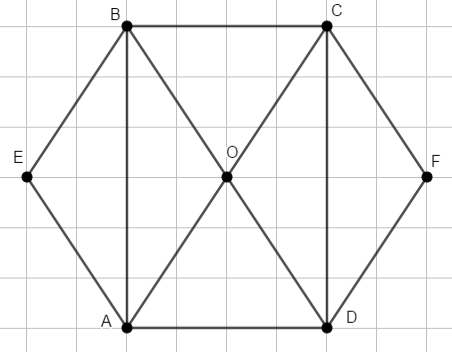
\includegraphics[width=0.9\linewidth]{cflash_7.png}
% % 	\end{center}
% % 	\end{minipage}
% % \end{exercice}


\end{document}